\documentclass[letterpaper]{article}

%%%% ========== PAQUETES NECESARIOS ========== %%%%
\usepackage[utf8]{inputenc} % Codificación de caracteres
\usepackage[spanish]{babel} % Idioma del documento
\usepackage[dvipsnames]{xcolor} % Colores extendidos
\usepackage{amsmath, amssymb, physics} % Matemáticas avanzadas
\usepackage{graphicx} % Insertar imágenes
\usepackage{multicol} % Múltiples columnas
\usepackage{tikz} % Dibujos vectoriales
\usetikzlibrary{arrows.meta, positioning}
\usepackage{fancyhdr} % Encabezados y pies de página
\usepackage[colorlinks=true, linkcolor=black,citecolor=black, urlcolor=black]{hyperref} % Hipervínculos
\usepackage[numbers, square]{natbib} % Citas y bibliografía
%%%% ========== CONFIGURACIÓN DE MÁRGENES ========== %%%%
\usepackage{geometry}
\geometry{bottom=2.54cm, top=2.54cm, left=2.54cm, right=2.54cm}

\usepackage{float}
\usepackage{booktabs}
%%%% ========== ENCABEZADOS Y PIES DE PÁGINA ========== %%%%
\pagestyle{fancy}
\fancyhf{}
\fancyhead[R]{Mecánica Estadística}
\fancyhead[L]{\thepage}
\renewcommand{\headrulewidth}{0.08pt}
\renewcommand{\footrulewidth}{0.08pt}
\fancyfoot[L]{}
\fancyfoot[R]{\rightmark}

%%%% ========== COMANDOS PERSONALIZADOS ========== %%%%
\newcommand{\Title}[1]{\begin{center}\LARGE\textbf{\textit{#1}}\end{center}}
\newcommand{\Abstract}[1]{\begin{abstract}\normalsize{#1}\end{abstract}}
\newcommand{\Theorem}[1]{\begin{center}\normalsize\textit{#1}\end{center}}

% Colores personalizados
\newcommand{\blue}{\color{blue}}
\newcommand{\red}{\color{red}}
\newcommand{\green}{\color{OliveGreen}}
\newcommand{\orange}{\color{orange}}

% Atajos matemáticos
\newcommand{\Identity}{\mathbb{I}}
\newcommand{\Reals}{\mathbb{R}}
\newcommand{\Naturals}{\mathbb{N}}
\newcommand{\Integers}{\mathbb{Z}}
\newcommand{\Complex}{\mathbb{C}}

% Operadores matemáticos
\newcommand{\Grad}{\vec{\nabla}}
\newcommand{\Divg}{\vec{\nabla} \cdot}
\newcommand{\Curl}{\vec{\nabla} \times}
\newcommand{\Lapl}{\nabla^{2}}

% Derivadas y operadores
\newcommand{\Partial}[2]{\frac{\partial#1}{\partial#2}}
\newcommand{\SecPartial}[3]{\frac{\partial^{2}#1}{\partial#2\partial#3}}

% Ecuaciones de movimiento
\newcommand{\eqLagrange}[1]{\frac{d}{dt}\cbk{\Partial[\dot{#1}]{\Lag}} - \Partial[#1]{\Lag} = 0}
\newcommand{\Ham}{\mathcal{H}}
\newcommand{\eqHamilton}[2]{\Partial[#1_{i}]{\Ham} = - \dot{#2}_{i}, \quad \Partial[#2_{i}]{\Ham} = \dot{#1}_{i}}

\setlength{\parindent}{0pt}
\setlength{\parskip}{1em} 

\begin{document}

\Title{Redes Neuronales: Sistemas complejos y aplicaciones.}
\Abstract{Hola :p \citep{dieckman2005} asi se cita}

\setlength{\parindent}{1.5em}
\setlength{\parskip}{0pt}
\tableofcontents
\clearpage

\section*{Objetivos}
\section{Redes neuronales biológicas vs redes neuronales artificiales}
\label{sec_intro}

\subsection{Funcionamiento de neuronas biológicas}

Del marco de trabajo de la termodinámica se ha aprendido a trabajar con modelos empíricos, es decir modelos que responden a la experiencia fenomenológica, desde esta forma de trabajar, se puede intentar replicar la forma en la que naturaleza se comporta en sistemas como el cerebro, lo cual se tratará de hacer utilizando redes neuronales artificiales. La obra maestra de la naturaleza son las redes neuronales biológicas. El cerebro humano está conformado por billones de neuronas, en las que cada una de ellas se conecta a miles de otras, lo que genera una compleja red para manejar información. Una neurona es una célula nerviosa que tiene la función de recibir, procesar y transmitir información por medio de señales eléctricas y químicas, debido a la excitabilidad eléctrica (capacidad de las neuronas de cambiar su potencial eléctrico y transmitir este cambio a través de su axón) de su membrana plasmática. \  

Una neurona biológica tiene tres partes principales: 
\begin{enumerate}
\item Dendritas: Reciben las señales de otras neuronas.
\item Cuerpo celular (soma): Procesan las señales entrantes.  
\item Axón: Es la parte que conduce impulsos eléctricos desde el cuerpo celular hacia otras neuronas. 
\end{enumerate} 

\begin{figure}[h!] %H para ocupar imagenes en doble col.
		\centering	
		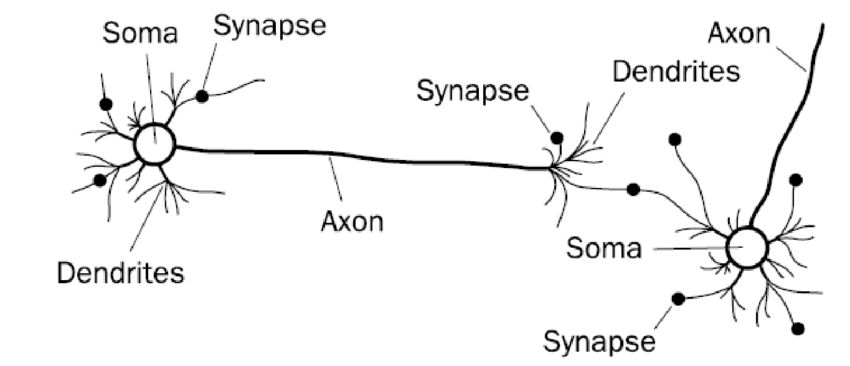
\includegraphics[scale=0.25]{Biological-neural-network-2}
		\caption{Representación de una neurona}
\end{figure}

\subsection{Transmisión de señales y mecanismos de aprendizaje}

Las neuronas se comunican mediante impulsos conocidos como potenciales de acción. Cuando una señal alcanza la parte final del axón, se liberan neurotransmisores transfiriendo la señal a la siguiente neurona. 

Las neuronas fortalecen o debilitan sus conexiones basándose en la experiencia, la plasticidad sináptica (capacidad del cerebro de modificar la fuerza o eficacia de las conexiones sinápticas entre neuronas) es el equivalente biológico al aprendizaje. 

Las redes neuronales biológicas son adaptativas, distribuibles 

\subsection{Funcionamiento de neuronas artificiales}

Una neurona artificial o perceptrón es la red neuronal más simple de todas ya que sólo contiene una única capa de entrada y un nodo de salida, es un modelo matemático simplificado para tratar de replicar el funcionamiento de una neurona biológica. Sus partes son: 

\begin{enumerate}
\item Entradas: Reciben señales como lo hacen las dendritas, con la diferencia de que las entradas de las neuronas artificiales son entradas numéricas.
\item Pesos sinápticos: Cada una de las entradas es ponderada, lo cual representa la fuerza de cada conexión.
\item Función de agregación: Las entradas ponderadas se suman. 
\item Función de activación: La suma pasa a través de una \textit{función de activación} que determina si la neurona da un valor de salida.
\item Salida: La salida final que pasa a la siguiente capa de neuronas. 
\end{enumerate}

\begin{figure}[h!] %H para ocupar imagenes en doble col.
		\centering	
		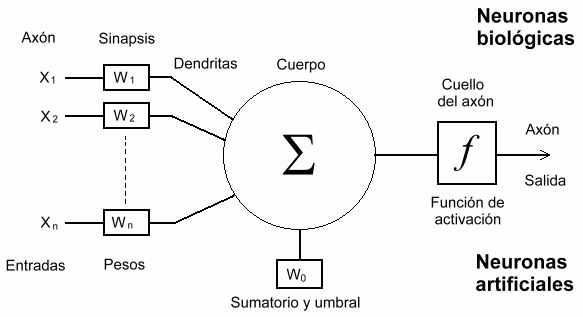
\includegraphics[scale=0.7]{artneuron.png}
		\caption{Neurona artificial}
\end{figure}

En la fig. 2 se puede ver en la parte inferior las partes que conforman la neurona artificial y en la parte superior a que corresponde esa parte en una neurona biológica.

\subsubsection{Modelo de McCulloch-Pitts}

El modelo más simple para una neurona artificial es el modelo de McCulloch-Pitts, modelo que se puede observar en la fig. 2, en este modelo las entradas son el estímulo que la neurona artificial recibe del entorno que le rodea, la salida es la respuesta a ese estímulo. En este modelo la neurona se adapta al medio y aprende de él modificando el valor de los pesos sinápticos, por lo cual los mismos serán los parámetros libres que ayudaran a optimizar el aprendizaje de la neurona. La salida neuronal está dada por 

\begin{equation}
Y=f( \omega_0 + \sum_{i=1}^n \omega_i x_i )
\end{equation}

donde $\omega_0$ es el umbral, $\omega_i x_i$ son las entradas $x_i$ siendo ponderadas por el peso $\omega_i$. La función del umbral es la de actuar como un valor constante que permite que la neurona se active o "dispare" incluso si la suma ponderada de las entradas es igual a cero. La función de activación suele elegirse de acuerdo a la tarea realizada por la neurona. En la siguiente tabla se muestran algunas funciones de activación utilizadas para diversos tipos de redes neuronales. 

\begin{figure}[h!] %H para ocupar imagenes en doble col.
		\centering	
		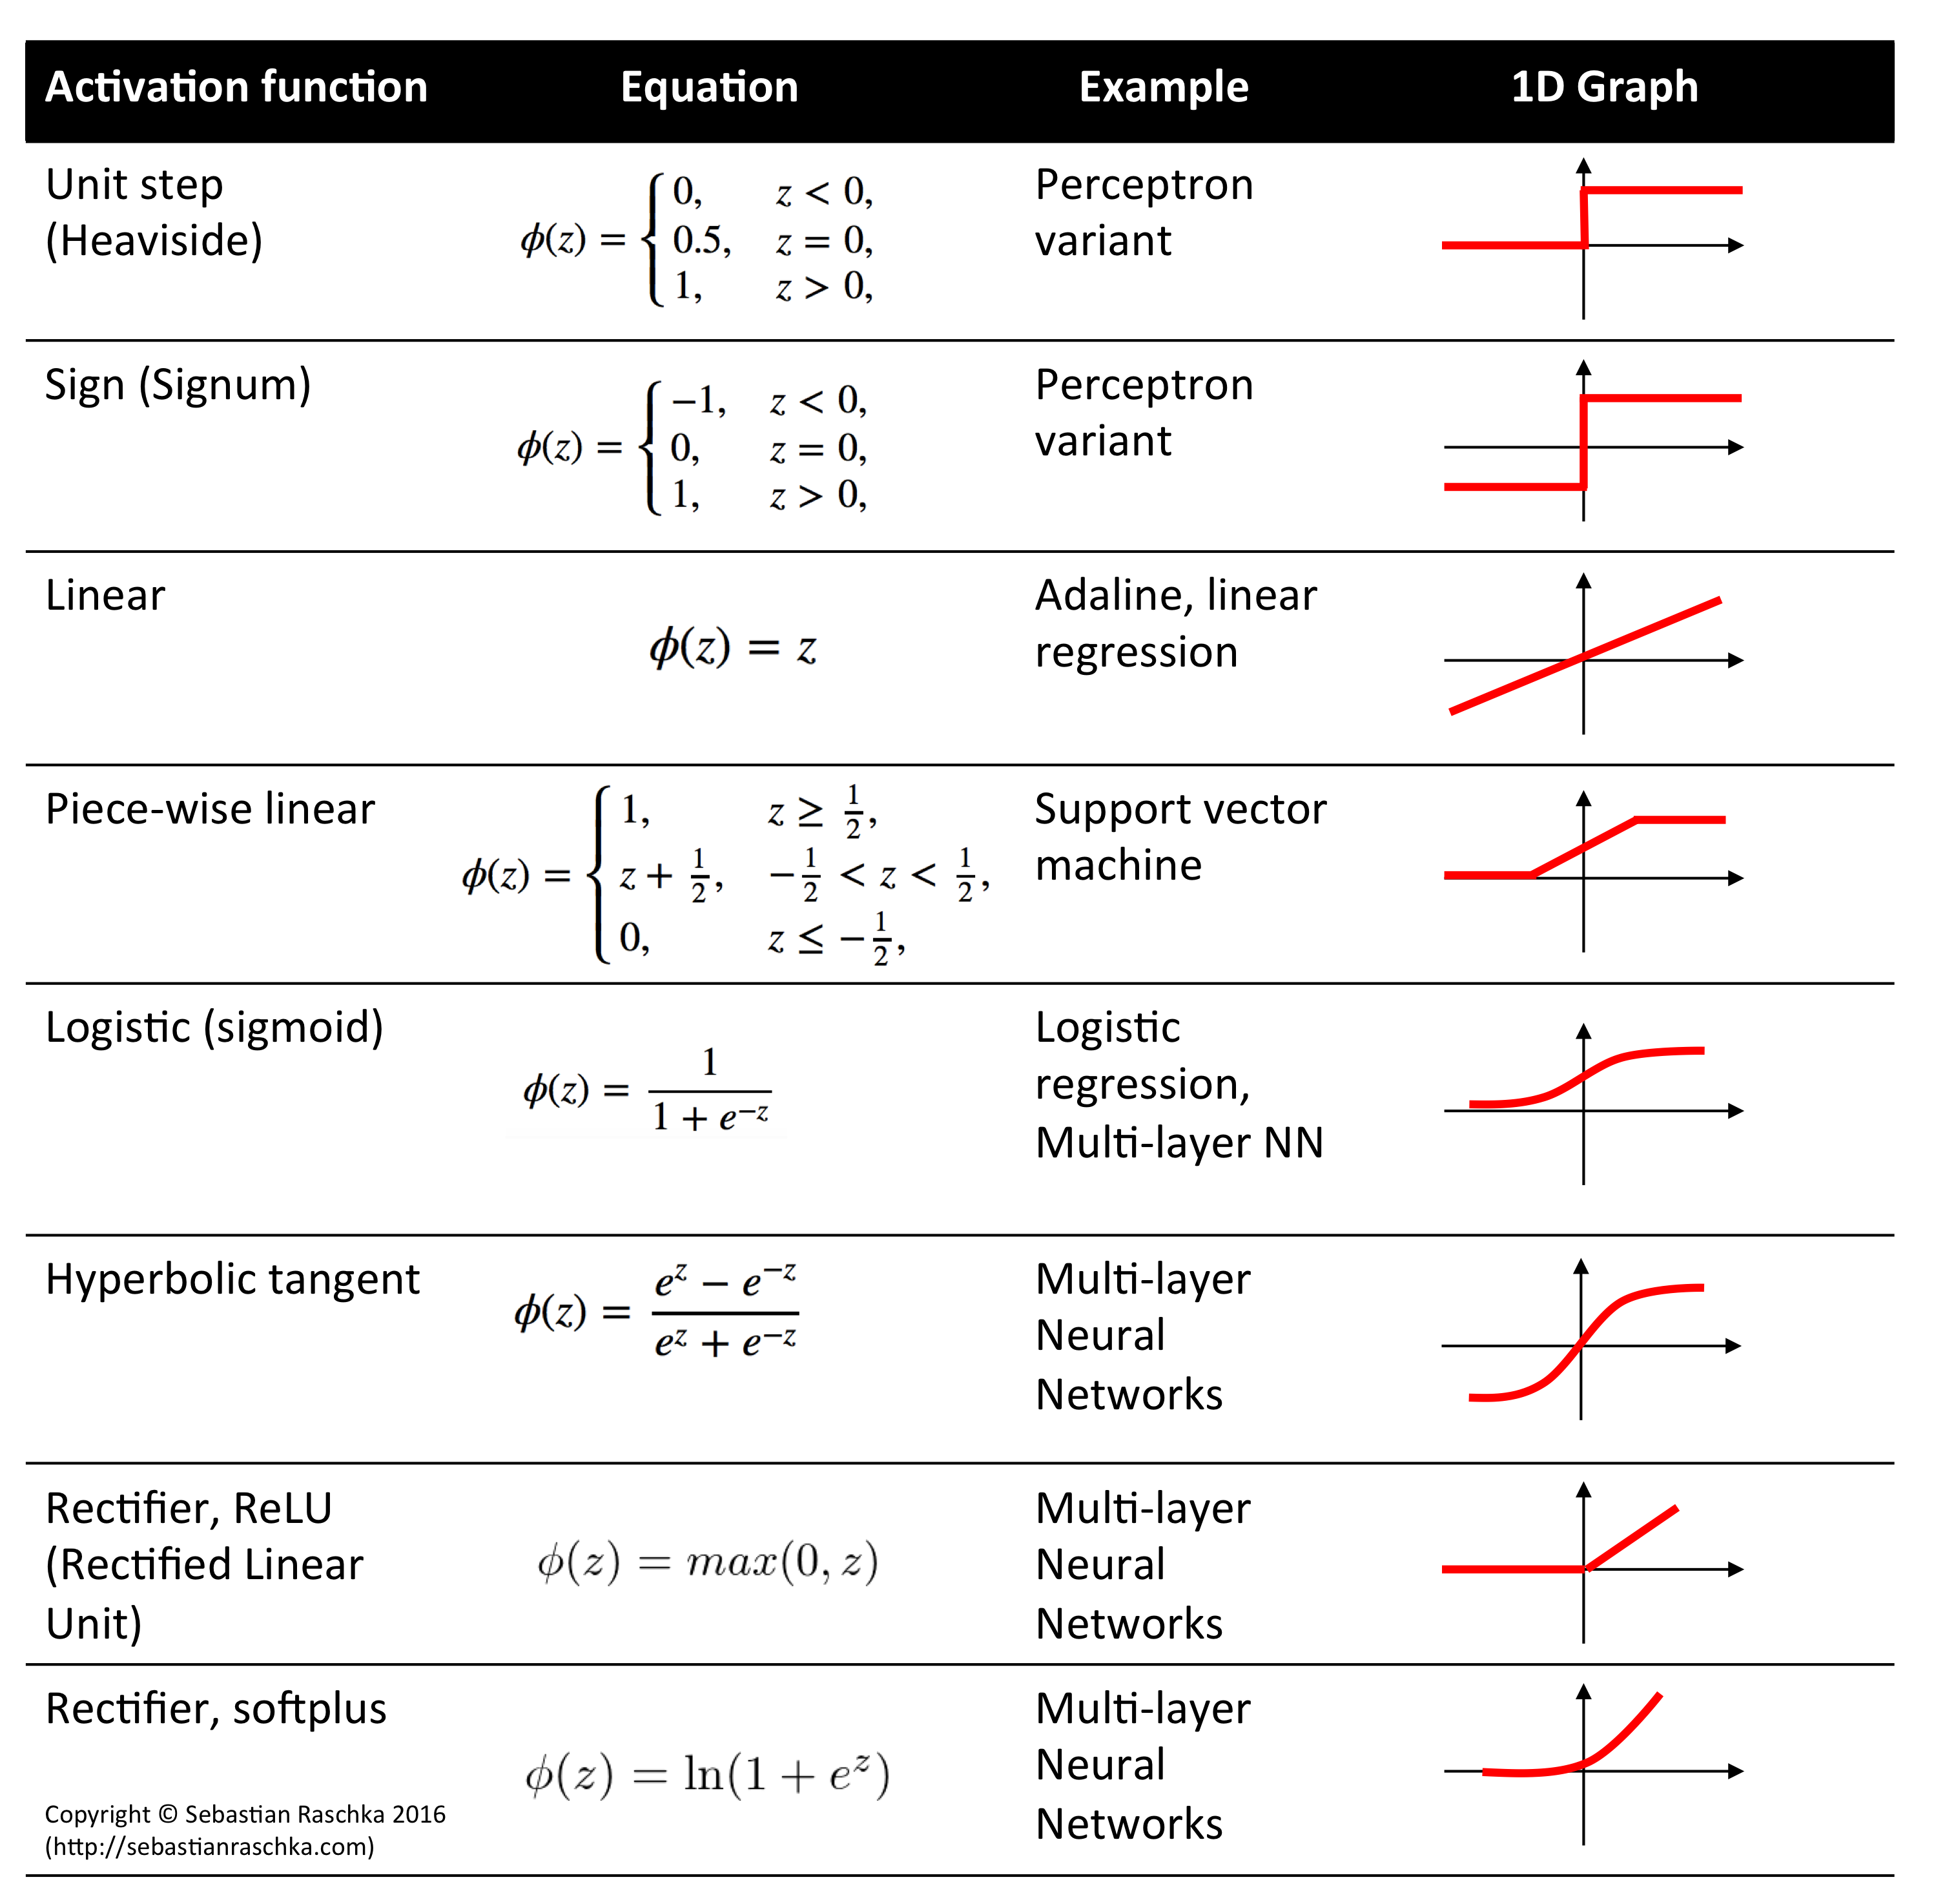
\includegraphics[scale=0.15]{activation-functions.png}
		\caption{Funciones de activación comunes}
\end{figure}

Como ejemplo se puede decir que una función de activación lineal se utiliza a la salida en redes neuronales que resuelven problemas de regresión. Compuertas del tipo signum o sigmoid se utilizan en redes neuronales que realizan procesos de clasificación binaria. 



\subsection{Diferencias clave entre redes neuronales biológicas y artificiales}

Así como una red neuronal biológica es un conjunto de neuronas interconectadas mediante la sinapsis, una red neuronal artificial es un conjunto de neuronas artificiales interconectadas. Por lo que, ahora que ya se conocen las partes que conforman una neurona artificial y una neurona biológica, se puede resumir en una tabla las principales diferencias una red neuronal biológica y una artificial. 


\begin{table}[h!]
\begin{center}
\begin{tabular}{| r | l | c |}
 & Redes Biológicas & Redes Artificiales \\ \hline
Componentes & Neuronas (dentritas, axones, sinapsis) & Nodos, pesos sinápticos \\
Tipo de Señal & Señales eléctricas y químicas & Datos numéricos \\
Aprendizaje & Plasticidad sináptica & Optimización del peso  \\ 
Adaptabilidad & Altamente adaptable y auto organizada & Requiere entrenamiento mediante datos \\
Rapidez & Lenta pero masivamente paralela & Rápida pero menos flexible  \\
Escala & Billones de neuronas & Pocos millones de nodos  \\ \hline
\end{tabular}
\caption{Diferencias entre redes biológicas y artificiales}
\label{tab:fruta}
\end{center}
\end{table} 

\subsection{Redes Neuronales Multicapa MLP}

Las redes neuronales multicapa contienen más de una capa computacional. El perceptrón contiene una capa de entrada y una capa de salida, de las cuales la capa de salida es la única capa que realiza cálculos. La capa de entrada transmite los datos hacia la capa de salida y todos los cálculos son visibles al usuario. Las redes neuronales multicapa contienen múltiples capas computacionales, capas intermedias adicionales entre la entrada y la salida a las cuales se les conoce como \textit{capas ocultas} debido a que los cálculos realizados en ellas no son visibles al usuario. La arquitectura específica de estas redes es de tipo prealimentado ó \textit{feed-forward}, en dicha arquitectura se asume que todos los nodos en cada capa están conectados a aquellos de la siguiente capa. Por lo tanto, la arquitectura de la red neuronal, estará casi definida, una vez que el número de capas y el número/tipo de nodos en cada capa se haya definido. Al número de unidades que tiene cada capa se le conoce como \textit{dimensionalidad} de la capa.

\begin{figure}[h!] %H para ocupar imagenes en doble col.
		\centering	
		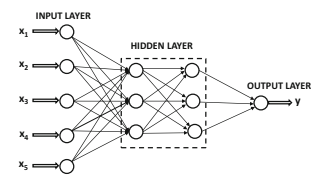
\includegraphics[scale=1]{redmulticapa.png}
		\caption{Red Multicapa}
\end{figure}

Se puede entender por lo tanto que la capa de entrada recibe los datos, la capa oculta procesa los datos y la capa de salida da la respuesta de la red. Este tipo de redes se ponen a prueba con datos estandarizados para ver la capacidad que tiene la red para reproducirlos, optimizando el proceso hasta lograr el resultado esperado, a esto se le conoce como \textit{entrenamiento} de la red.

\subsection{Redes Neuronales Convolucionales CNN}

Las redes neuronales convolucionales son redes inspiradas en redes biológicas y que se usan principalmente en visión computarizada para la clasificación y detección de objetos. La motivación básica para este tipo de redes se obtuvo del entendimiento que Hubel y Weisel lograron acerca de la corteza visual en los gatos, en la cual porciones específicas del campo visual excitan ciertas neuronas. 

Para las redes convolucionales, se define una \textit{operación de convolución}, en la cual se usa un filtro para mapear las activaciones de una capa a la siguiente. Una operación de convolución utiliza un filtro tridimensional de pesos con la misma profundidad que la capa en la que se encuentra pero con una medida espacial menor. El producto punto entre todos los pesos en el filtro y cualquier elección de región espacial (del mismo tamaño del filtro) en una capa define el valor del estado oculto en la siguiente capa. La operación entre el filtro y la región espacial en la capa se realiza en cada posición posible de modo que se pueda definir la siguiente capa.

\begin{figure}[h!] %H para ocupar imagenes en doble col.
		\centering	
		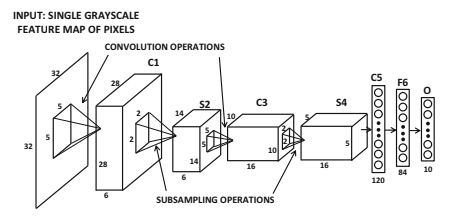
\includegraphics[scale=1]{redconvolucional.png}
		\caption{Una de las primeras redes convolucionales}
\end{figure}

Las redes neuronales convolucionales han sido las redes más exitosas de todos los tipos de redes neuronales. Se utilizan ampliamente para reconocimiento de imágenes, detección de objetos e incluso en procesamiento de texto. El desempeño de estas redes ha superado recientemente a los humanos en la realización de tareas de clasificación de imágenes, por esto pueden llegar a ser bastante útiles como herramienta para el diagnóstico de enfermedades basados en estudios de imagenología clínica. 

\subsection{Propiedades de una red compleja}

Es importante conocer e identificar las propiedades que tiene una red compleja como lo son las redes neuronales, desde este punto de vista, la teoría de grafos es una herramienta bastante poderosa para describir y cuantificar las propiedades de redes complejas. Propiedades como la densidad de nodos o el coeficiente de agrupamiento se utilizan en áreas como la neurociencia para relacionar la estructura cerebral con el comportamiento. Por lo tanto en la siguiente sección se iniciará un estudio de las bases teóricas de la teoría de grafos. 

\input{02_Fundamentos Teóricos.tex}
%\section{}
\section{Aplicaciones de las redes neuronales}
\subsection{Feedforward}
\begin{itemize}
    \item Estas redes son útiles para tareas en las que hay que aprender una relación entre entradas y salidas, típicamente:
    \item Clasificación de imágenes: Reconocimiento de productos, detección de defectos en imágenes.
    \item Predicción de series temporales: Pronósticos de ventas, análisis del mercado bursátil, gestión energética.
    \item Detección de fraudes: Identificación de transacciones fraudulentas en tarjetas de crédito.
\end{itemize}
\subsection{Redes Neuronales Recurrentes (RNN)}
Permiten procesar secuencias de datos, ya que la información se retroalimenta a través de bucles en la red.

Se usan comúnmente para problemas ordinarios o temporales como, por ejemplo, la traducción de idiomas, el procesamiento del lenguaje natural (NLP), el reconocimiento de voz y los subtítulos de imágenes; se incorporan a aplicaciones populares como Siri y Google Translate.

Algunas aplicaciones típicas:
Traducción automática: Traducción de textos de un idioma a otro.

Reconocimiento de voz: Conversión de voz a texto.

Análisis de sentimientos: Detección de emociones en textos o publicaciones en redes sociales.
\subsection{Hopfield}
La Red de Hopfield es una red recurrente, es decir, existe realimentación entre las neuronas. De esta forma, al introducir un patrón de entrada, la información se propaga hacia adelante y hacia atrás, produciéndose una dinámica. En algún momento, la evolución se detendrá en algún estado estable. En otros casos, es posible que la red no se detenga nunca.

Las aplicaciones típicas de las Redes Hopfield incluyen el reconocimiento de patrones, la memoria direccionable por contenido y la optimización .

\section{Red neuronal convolucional para la detección y clasificación del cáncer de mama mediante aprendizaje profundo}
El estudio presenta una nueva arquitectura de CNN llamada BCCNN, diseñada para detectar y clasificar imágenes de cáncer de mama en ocho clases distintas (presumiblemente diferentes tipos o estados de tumores). El objetivo es mejorar la precisión y versatilidad en el diagnóstico, y demostrar que una CNN con mecanismos de regulación de aprendizaje puede alcanzar resultados clínicamente útiles \citep{abunasser2023cnn}.
\subsection{Datos y procesamiento}

Orígenes del dataset: Obtienen imágenes de mamografías a partir de bases públicas en Kaggle (como CBIS-DDSM, MiniDDSM y otras) .
Estas bases incluyen imágenes originales junto con etiquetas clínicas (benigno, maligno, subcategorías).

Preprocesamiento:
Normalización del tamaño y contraste.
Aumento de datos: rotaciones, espejos y escalados para ampliar el set y evitar sobreajuste.

\textbf{Clases de tumeres identificadas:}
\begin{itemize}
    \item BA (adenosis benigno)
    \item BF (fibroadenoma benigno)
    \item BPT (tumor benigno de phyllodes)
    \item BTA (adenoma tubular benigno)
    \item MDC (carcinoma ductal maligno)
    \item MLC (carcinoma lobular maligno)
    \item MMC (carcinoma mucinoso maligno)
    \item MPC (carcinoma papilar maligno)
\end{itemize}
\begin{figure}
    \centering
    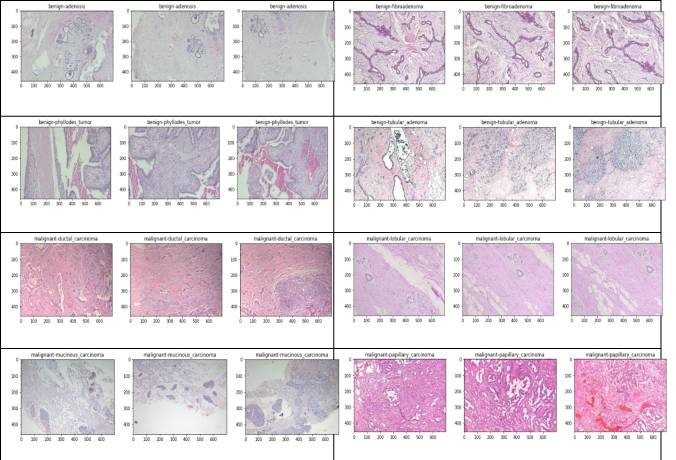
\includegraphics[width=0.5\linewidth]{cancer.jpg}
    \caption{}
    \label{fig:enter-label}
\end{figure}


\subsection{Arquitectura}
\begin{itemize}
    \item Entrada

Imagen de RM (resonancia) con distintas magnificaciones (40x–400x).

\item Capas Convolucionales 
Varias capas CNN que extraen características visuales progresivas (texturas, formas).

No se especifican filtros exactos, pero siguen un patrón típico de extracción jerárquica.

\item Pooling

Capas de max pooling para reducir la información espacial y concentrar lo relevante.

\item Flatten

Convierte los mapas de características en un vector 1D.

\item Capas Fully Connected

Una o más capas densas que combinan las características para clasificación.

\item Capa de salida (Softmax)

8 neuronas (una por clase), con función softmax para obtener la probabilidad de cada tumor.


    
\end{itemize}
\subsection{Comparación con otros modelos}
El artículo también evalúa y compara BCCNN con seis modelos pre-entrenados en ImageNet:

Xception,InceptionV3,VGG16,MobileNet,ResNet50.

Realizan un total de 30 experimentos, combinando los seis modelos con las cinco magnificaciones de imagenes (40x–400x)
\subsection{Resultados}
F1-score del BCCNN: $98.28\%.$

Comparado con los demás:

ResNet50: $98.14\%$

VGG16: $97.67\%$

Xception: $97.54\%$

MobileNet: $93.98\%$

Esto muestra que su arquitectura personalizada logró resultados ligeramente mejores que modelos grandes preentrenados .


\section{Conclusiones}
A través de este estudio, hemos observado cómo la estructura de las redes neuronales y si dinámica pueden modelarse y analizarse utilizando herramientas de distintas disciplinas. La comparación entre redes artificiales y biológicas nos da mas claridad en los retos y oportunidades que nos da la inteligencia artificial.

La exploración de los distintos tipos de de redes demuestran la importancia de la conectividad para determinar el comportamiento de una red. Además, las diversas aplicaciones de estas redes que abarcan desde el aprendizaje automático hasta los sistemas biológicos y sociales dan indicios de su uso para nuevas y mejores tecnologías.

Las redes neuronales son una gran herramienta para comprender sistemas complejos y ofrecen nuevas técnicas en la investigación teórica y la aplicada. Los futuros avances en este campo profundizarán nuestra comprensión de sistemas más complejos y mas realistas, proporcionado el camino para soluciones innovadoras a problemas del mundo real.


\clearpage
\bibliographystyle{plainnat}
\bibliography{ref}
\end{document}
